\documentclass{standalone}
\usepackage{tikz}
\usetikzlibrary{calc}
\begin{document}
    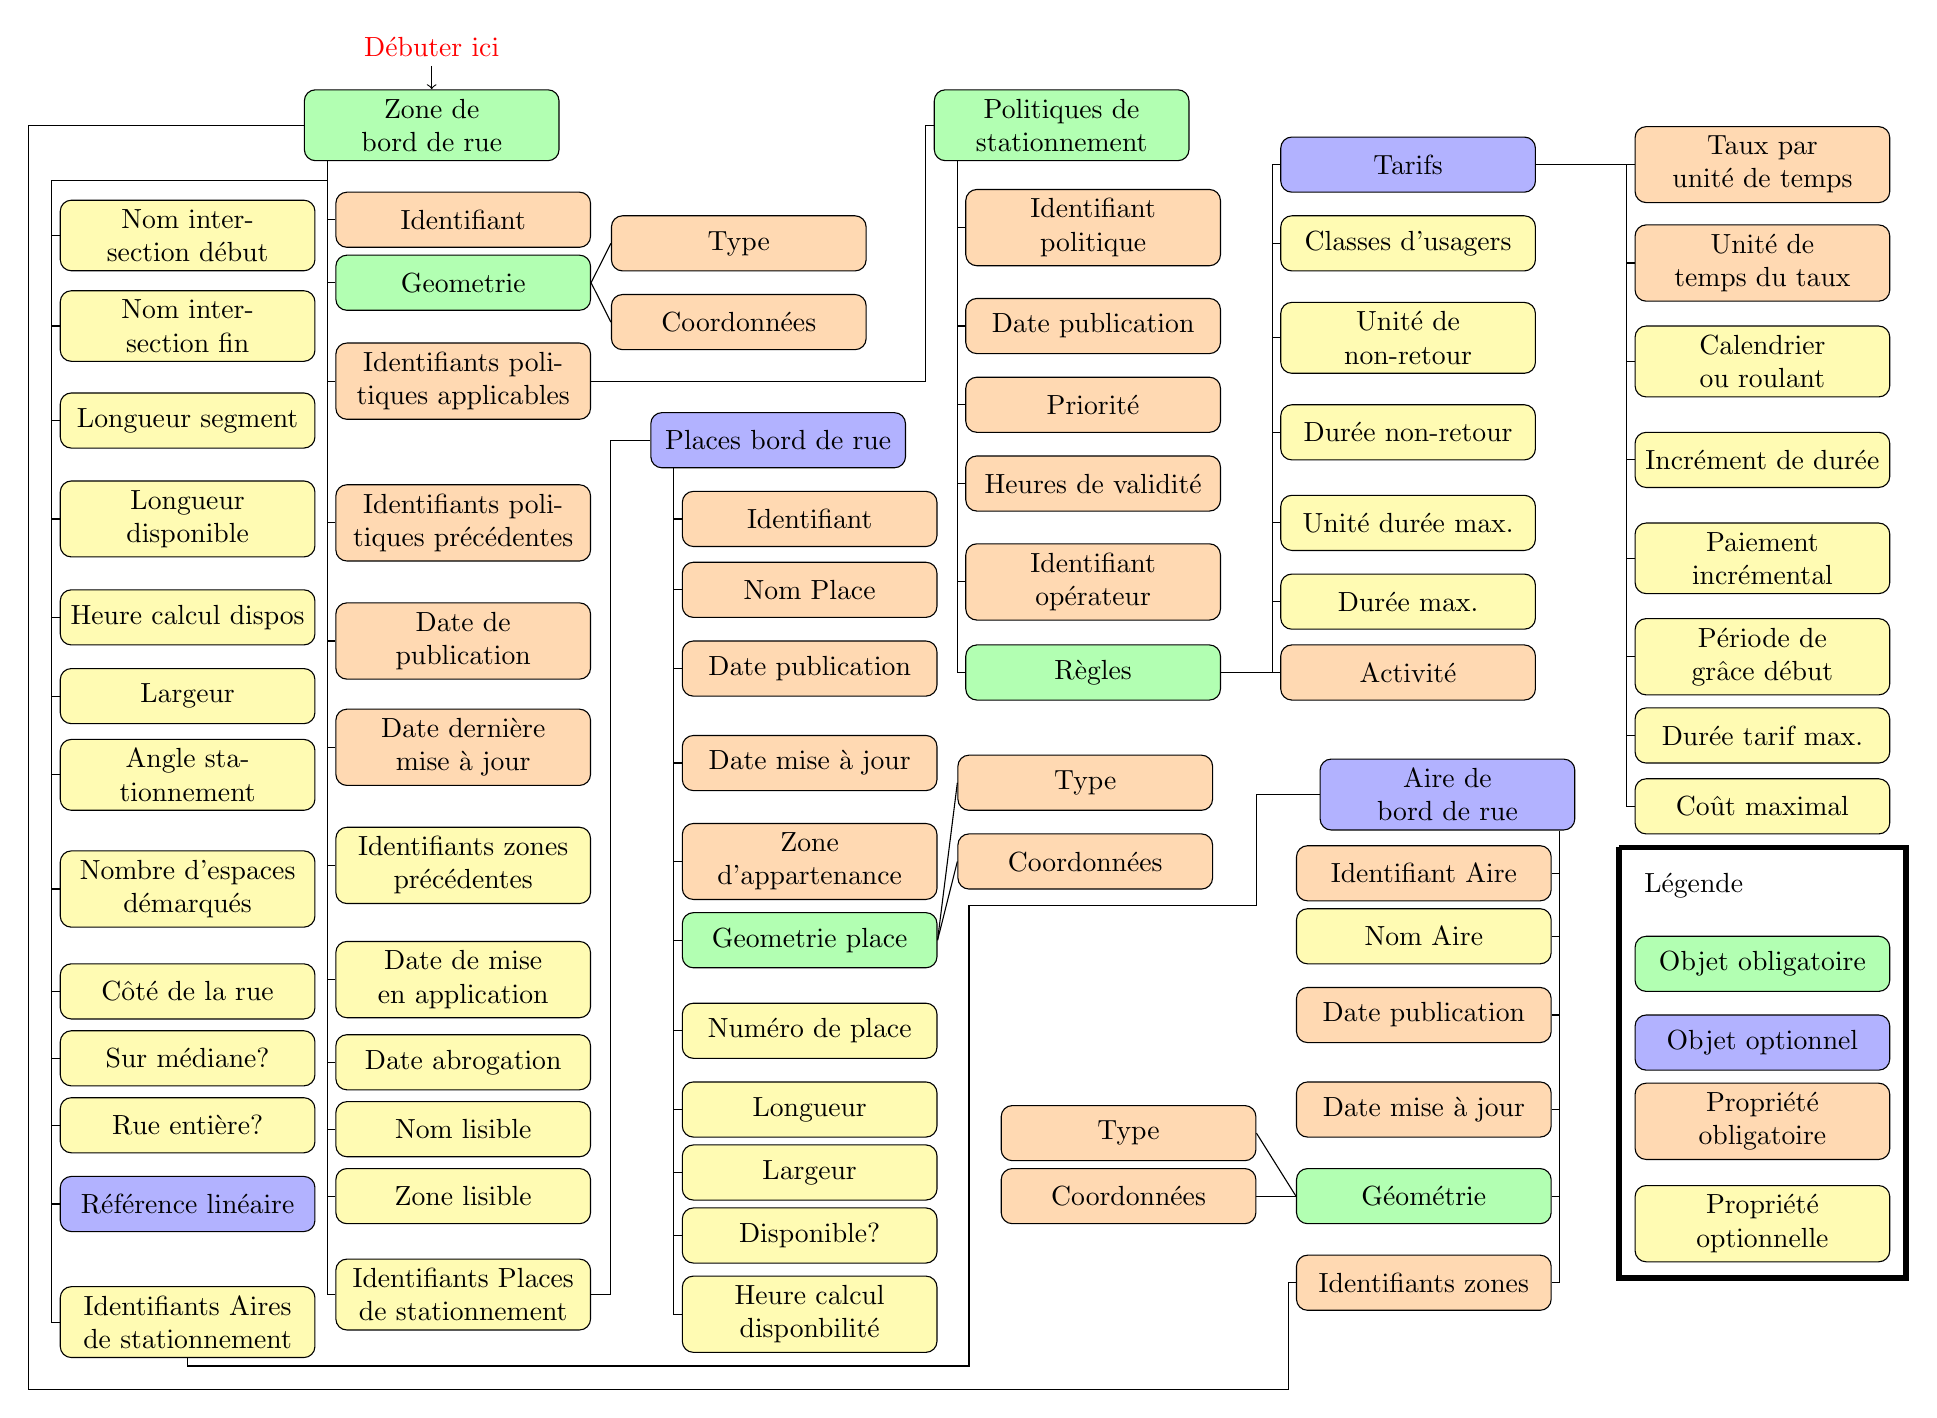
\begin{tikzpicture}
        \tikzstyle {objet} = [rectangle, rounded corners, text width=3cm, minimum height=0.7cm,text centered,  draw=black, fill=green!30]
        \tikzstyle {objet_opt} = [rectangle, rounded corners, text width=3cm, minimum height=0.7cm,text centered,  draw=black, fill=blue!30]
        \tikzstyle {propriete} = [rectangle, rounded corners, text width=3cm, minimum height=0.7cm,text centered,  draw=black, fill=orange!30]
        \tikzstyle{propriete_opt} =[rectangle, rounded corners, text width=3cm, minimum height=0.7cm,text centered,  draw=black, fill=yellow!30]
        % Zone de stationnement
        
        \node (zone)[objet]{Zone de bord de rue};
        \node (debut)[above of=zone,color=red]{Débuter ici};
        \draw [->](debut.south) --(zone.north);
        
            % Colonne droit
            \node (identifiant)[propriete, below of=zone,xshift=0.4cm,yshift=-0.2cm]{Identifiant};
            \coordinate (joint) at ($ (identifiant.west) + (-0.1,0.5) $);
            \draw (identifiant.west) -| (joint) |- ($(zone.south -|joint)$);
            \node (geometrie) [objet, below of=identifiant,yshift=0.2cm]{Geometrie};
            \draw (geometrie.west) -| ++(-0.1,0.1) |- (identifiant.west);
            \node (type) [propriete,right of=geometrie,xshift=2.5cm,yshift=0.5cm]{Type};
            \draw (type.west) -- (geometrie.east);
            \node (coordonnees) [propriete,below of=type]{Coordonnées};
            \draw (coordonnees.west) -- (geometrie.east);
            \node (politiques) [propriete, below of=geometrie,yshift=-0.25cm]{Identifiants politiques applicables};
            \draw (politiques.west) -| ++(-0.1,0.1) |- (geometrie.west);
            \node (politiques_precedentes) [propriete, below of=politiques,yshift=-0.8cm]{Identifiants politiques précédentes};
            \draw (politiques_precedentes.west) -| ++(-0.1,0.1) |- (politiques.west);
            \node (date_publication) [propriete, below of=politiques_precedentes,yshift=-0.5cm]{Date de publication};
            \draw (date_publication.west) -| ++(-0.1,0.1) |-(politiques_precedentes.west);
            \node (date_maj) [propriete,below of=date_publication,yshift=-0.35cm]{Date dernière mise à jour};
            \draw (date_maj.west) -| ++(-0.1,0.1) |- (date_publication.west);
            \node (zones_precedentes) [propriete_opt, below of=date_maj,yshift=-0.5cm] {Identifiants zones précédentes};
            \draw (zones_precedentes.west) -| ++(-0.1,0.1) |- (date_maj.west);
            \node (date_debut) [propriete_opt,below of=zones_precedentes,yshift=-0.45cm] {Date de mise en application};
            \draw (date_debut.west) -| ++(-0.1,0.1) |- (zones_precedentes.west);
            \node (date_fin) [propriete_opt, below of=date_debut,yshift=-0.05cm]{Date abrogation};
            \draw (date_fin.west) -| ++(-0.1,0.1) |-(date_debut.west);
            \node (nom) [propriete_opt,below of=date_fin,yshift=0.15cm]{Nom lisible};
            \draw (nom.west) -| ++(-0.1,0.1) |- (date_fin.west) ;
            \node (zone_identifiant) [propriete_opt, below of=nom,yshift=0.15cm]{Zone lisible};
            \draw (zone_identifiant.west) -| ++(-0.1,0.1) |- (nom.west);
            \node (ids_places) [propriete_opt,below of=zone_identifiant,yshift=-0.25cm]{Identifiants Places de stationnement};
            \draw (ids_places.west) -| ++(-0.1,0.1) |- (zone_identifiant.west);
            
            % Colonne gauche
            \node (nom_intersection_debut) [propriete_opt,left of=identifiant,xshift=-2.5cm,yshift=-0.2cm]{Nom intersection début};
            \draw (nom_intersection_debut.west) -| ++(-0.1,0.1) |- (joint);
            \node (nom_intersection_fin) [propriete_opt,below of=nom_intersection_debut,yshift=-0.15cm]{Nom intersection fin};
            \draw (nom_intersection_fin.west) -| ++(-0.1,0.1) |- (nom_intersection_debut.west);
            \node (longueur) [propriete_opt,below of=nom_intersection_fin,yshift=-0.2cm]{Longueur segment};
            \draw (longueur.west) -| ++(-0.1,0.1) |- (nom_intersection_fin.west);
            \node (longueurs_dispo)[propriete_opt, below of=longueur,yshift=-0.25cm]{Longueur disponible};
            \draw (longueurs_dispo.west) -| ++(-0.1,0.1) |-(longueur.west) ;
            \node (heure_dispo_calcul)[propriete_opt,below of=longueurs_dispo,yshift=-0.25cm]{Heure calcul dispos};
            \draw (heure_dispo_calcul.west) -| ++(-0.1,0.1) |- (longueurs_dispo.west);
            \node (largeur) [propriete_opt,below of=heure_dispo_calcul]{Largeur};
            \draw (largeur.west) -| ++(-0.1,0.1) |- (heure_dispo_calcul.west);
            \node (parking_angle)[propriete_opt,below of=largeur]{Angle stationnement};
            \draw (parking_angle.west) -| ++(-0.1,0.1) |- (largeur.west);
            \node (num_espaces) [propriete_opt,below of=parking_angle,yshift=-0.45cm]{Nombre d'espaces démarqués};
            \draw (num_espaces.west) -| ++(-0.1,0.1) |- (parking_angle.west);
            \node (cote_rue) [propriete_opt,below of=num_espaces,yshift=-0.3cm]{Côté de la rue};
            \draw (cote_rue.west) -| ++(-0.1,0.1) |- (num_espaces.west);
            \node (mediane) [propriete_opt,below of=cote_rue,yshift=0.15cm]{Sur médiane?};
            \draw (mediane.west) -| ++(-0.1,0.1) |- (cote_rue.west);
            \node (rue_complete) [propriete_opt,below of=mediane,yshift=0.15cm]{Rue entière?};
            \draw (rue_complete.west) -| ++(-0.1,0.1) |- (mediane.west);
            \node (ref_lineaire) [objet_opt,below of=rue_complete]{Référence linéaire};
            \draw (ref_lineaire.west) -| ++(-0.1,0.1) |- (rue_complete.west);
            \node (ids_aires) [propriete_opt, below of=ref_lineaire,yshift=-0.5cm]{Identifiants Aires de stationnement};
            \draw (ids_aires.west) -| ++(-0.1,0.1) |- (ref_lineaire.west);
            \coordinate (enter_aire) at ($(ids_aires.south) + (0.1,-0.1)$);
            \coordinate (double_enter_aire) at ($(ids_aires.south) + (0,-0.4)$);
            \coordinate (triple_enter_aire) at ($(ids_aires.west) + (-0.4,0)$);
        % Places de bord de rue
        \node (place) [objet_opt,below of=coordonnees,xshift=0.5cm,yshift=-0.5cm]{Places bord de rue};
        \draw (ids_places.east) -| ++(0.25,0.25) |- (place.west);
            % Colonne
            \node (ids_places_objet) [propriete, below of=place,xshift=0.4cm]{Identifiant};
            \draw (ids_places_objet.west) -| ++(-0.1,0.1) |-($(ids_places_objet.west |- place.south) + (-0.1,0)$);
            \node (nom_place) [propriete, below of=ids_places_objet,yshift=0.1cm]{Nom Place};
            \draw (nom_place.west) -| ++(-0.1,0.1) |- (ids_places_objet.west);
            \node (date_publie_place) [propriete, below of=nom_place]{Date publication};
            \draw (date_publie_place.west) -| ++(-0.1,0.1) |- (nom_place.west);
            \node (date_changement_place) [propriete, below of=date_publie_place,yshift=-.2cm]{Date mise à jour};
            \draw (date_changement_place.west) -| ++(-0.1,0.1) |- (date_publie_place.west);
            \node (ident_match_place_zone) [propriete, below of=date_changement_place,yshift=-0.25cm]{Zone d'appartenance};
            \draw (ident_match_place_zone.west) -| ++(-0.1,0.1) |- (date_publie_place.west);
            \node (geometrie_place) [objet,below of=ident_match_place_zone]{Geometrie place};
            \draw (geometrie_place.west) -|++(-0.1,0.1) |- (ident_match_place_zone.west);
            \node (type_place) [propriete,right of=geometrie_place,xshift=2.5cm,yshift=2cm]{Type};
            \draw (type_place.west) -- (geometrie_place.east);
            \node (coordonnees_place) [propriete,below of=type_place]{Coordonnées};
            \draw (coordonnees_place.west) -- (geometrie_place.east);
            \node (space_number) [propriete_opt,below of=geometrie_place,yshift=-0.15cm]{Numéro de place};
            \draw (space_number.west) -| ++(-0.1,0.1) |- (geometrie_place.west);
            \node (length) [propriete_opt, below of=space_number]{Longueur};
            \draw (length.west) -| ++(-0.1,0.1) |- (space_number.west);
            \node (width) [propriete_opt, below of=length,yshift=0.2cm]{Largeur};
            \draw (width.west) -| ++(-0.1,0.1) |- (length.west);
            \node (available) [propriete_opt, below of=width,yshift=0.2cm]{Disponible?};
            \draw (available.west) -| ++(-0.1,0.1) |- (width.west);
            \node (available_time) [propriete_opt, below of=available]{Heure calcul disponbilité};
            \draw (available_time.west) -| ++(-0.1,0.1) |- (available.west);
            \coordinate (coordonnees_bump) at ($(coordonnees_place.south)+ (-1,-0.2)$);
            \coordinate (coordonnees_bump_2) at ($(space_number.east) + (0.4,0)$);
        % Politiques de stationnement
        \node (politiques_obj) [objet,right of=zone,xshift=7cm]{Politiques de stationnement};
        \draw (politiques_obj.west) -|++(-0.1,-.01)|-(politiques.east);
            \node (ids_politiques) [propriete,below of=politiques_obj,xshift=0.4cm,yshift=-0.3cm] {Identifiant politique};
            \draw (ids_politiques.west) -| ++(-0.1,0.1) |- ($(politiques_obj.south-|ids_politiques.west)+(-0.1,0)$);
            \node (date_publication_politique) [propriete, below of=ids_politiques,yshift=-0.25cm]{Date publication};
            \draw (date_publication_politique.west) -| ++(-0.1,0.1) |- (ids_politiques.west);
            \node (priorite) [propriete,below of=date_publication_politique]{Priorité};
            \draw (priorite.west) -| ++(-0.1,0.1) |- (date_publication_politique.west);
            \node (heures_validite) [propriete, below of=priorite]{Heures de validité};
            \draw (heures_validite.west) -| ++(-0.1,0.1) |- (priorite.west);
            \node (ids_operateur) [propriete, below of=heures_validite,yshift=-0.25cm]{Identifiant opérateur};
            \draw (ids_operateur.west) -| ++(-0.1,0.1) |- (heures_validite.west);
            \node (regles) [objet,below of=ids_operateur,yshift=-0.15cm]{Règles};
            \draw (regles.west) -| ++(-0.1,0.1) |- (priorite.west);
        % Règles
            \node (activite) [propriete, right of=regles,xshift=3cm]{Activité};
            \draw (activite.west) -- (regles.east);
            \node (duree_max) [propriete_opt, above of=activite,yshift=-0.1cm]{Durée max.};
            \draw (duree_max.west) -| ++(-0.1,0.1) |- (activite.west);
            \node (unite_duree_max) [propriete_opt, above of=duree_max]{Unité durée max.};
            \draw (unite_duree_max.west) -| ++(-0.1,0.1) |- (duree_max.west);
            \node (no_return) [propriete_opt, above of=unite_duree_max,yshift=0.15cm]{Durée non-retour};
            \draw (no_return.west) -| ++(-0.1,0.1) |- (unite_duree_max.west);
            \node (unite_non_retour) [propriete_opt, above of=no_return,yshift=0.2cm]{Unité de non-retour};
            \draw (unite_non_retour.west) -| ++(-0.1,0.1) |- (no_return.west);
            \node (classes_usagers) [propriete_opt, above of=unite_non_retour,yshift=0.2cm]{Classes d'usagers};
            \draw (classes_usagers.west) -| ++(-0.1,0.1) |- (unite_non_retour.west);
            \node (tarifs) [objet_opt, above of=classes_usagers]{Tarifs};
            \draw (tarifs.west) -| ++(-0.1,-0.1) |- (classes_usagers.west); 
        % Tarifs
                \node (taux) [propriete, right of=tarifs,xshift=3.5cm]{Taux par unité de temps};
                \draw (tarifs.east) -- (taux.west);
                \node (taux_unite) [propriete, below of=taux,yshift=-0.25cm]{Unité de temps du taux};
                \draw (taux_unite.west) -| ++(-0.1,0.1) |- (taux.west);
                \node (rate_unit_period) [propriete_opt, below of=taux_unite,yshift=-0.25cm]{Calendrier ou roulant};
                \draw (taux_unite.west) -| ++(-0.1,0.1) |- (rate_unit_period.west);
                \node (increment_duration) [propriete_opt,below of=rate_unit_period,yshift=-0.25cm]{Incrément de durée};
                \draw (rate_unit_period.west) -| ++(-0.1,0.1) |- (increment_duration.west);
                \node (increment_valeur) [propriete_opt, below of=increment_duration,yshift=-0.25cm]{Paiement incrémental};
                \draw (increment_valeur.west) -| ++(-0.1,0.1) |- (increment_duration.west);
                \node (start_duration) [propriete_opt, below of=increment_valeur,yshift=-0.25cm]{Période de grâce début};
                \draw (start_duration.west) -| ++(-0.1,0.1) |- (increment_valeur.west);
                \node (end_duration) [propriete_opt, below of=start_duration]{Durée tarif max.};
                \draw (end_duration.west) -| ++(-0.1,0.1) |- (start_duration.west);
                \node (cout_max) [propriete_opt, below of=end_duration,yshift=0.1cm]{Coût maximal};
                \draw (cout_max.west) -| ++(-0.1,0.1) |- (end_duration.west);
        % Aires de bords de rue.
        \node (aire) [objet_opt,below of=tarifs,yshift=-7cm,xshift=0.5cm]{Aire de bord de rue};
            \node (id_aire) [propriete, below of=aire,xshift=-0.3cm]{Identifiant Aire};
            \draw (id_aire.east) -| ++(0.1,0.1) |-($(aire.south-|id_aire.east) + (0.1,0)$);
            \node (nom_aire) [propriete_opt, below of=id_aire,yshift=0.2cm]{Nom Aire};
            \draw (nom_aire.east) -| ++(0.1,0.1) |-(id_aire.east) ;
            \node (date_publication_aire) [propriete, below of=nom_aire]{Date publication};
            \draw (date_publication_aire.east)-| ++(0.1,0.1) |-(nom_aire.east);
            \node (date_maj_aire) [propriete, below of=date_publication_aire,yshift=-0.2cm]{Date mise à jour};
            \draw (date_maj_aire.east) -| ++(0.1,0.1) |-(date_publication_aire.east);
            \node (geometrie_aire) [objet,below of=date_maj_aire,yshift=-0.1cm]{Géométrie};
            \draw (geometrie_aire.east) -| ++(0.1,0.1) |- (date_maj_aire.east);
            \node (coordonnees_aire) [propriete, left of=geometrie_aire,xshift=-2.75cm]{Coordonnées};
            \node (type_geo_aire) [propriete, above of=coordonnees_aire,yshift=-0.2cm]{Type};
            \draw (coordonnees_aire.east) -- (geometrie_aire.west);
            \draw (type_geo_aire.east) -- (geometrie_aire.west);
            \node (identifiant_zones) [propriete, below of=geometrie_aire,yshift=-0.1cm]{Identifiants zones};
            \draw (identifiant_zones.east)  -| ++(0.1,0.1) |- (geometrie_aire.east);
        \draw (aire.west) -| ++(-0.8,-0.1) |- (coordonnees_bump) -| (coordonnees_bump_2) |- (enter_aire) -| (ids_aires.south);
        \draw (identifiant_zones.west) -|++(-0.1,-0.1) |- (double_enter_aire) -| (triple_enter_aire) |- (zone.west);
        \node (legend) [below of=cout_max, text width=3cm]{Légende};
        \coordinate (boite_top_left)at($(legend.north west)+ (-0.2,0.2)$);
        \node (objet_desc)[objet,below of=legend]{Objet obligatoire};
        \node (objet_opt_desc)[objet_opt,below of=objet_desc]{Objet optionnel};
        \node (propriete_desc) [propriete, below of= objet_opt_desc]{Propriété obligatoire};
        \node (prop_opt_desc) [propriete_opt, below of=propriete_desc,yshift=-.3cm]{Propriété optionnelle};
        \coordinate (boite_bot_rght) at ($(prop_opt_desc.south east)+ (0.2,-0.2)$);
        \draw[line width=2pt] (boite_top_left) -| (boite_bot_rght) -| (boite_top_left);
    \end{tikzpicture}
\end{document}